\newcommand{\Epsilon}{E}

\mysubsection{Commande Angulaire et Cartésienne}\label{Comm_Ang_e_Cart}
Pour développer les lois de commande pour le robot, on est parti de son modèle dynamique. L'idée principale est de contrôler la configuration angulaire du robot par le couple mécanique développé dans chaque articulation. Alors, la relation entre ces deux grandeurs est définie par le modèle dynamique direct:

	\begin{equation}
		\bm{\Gamma} = \bm{A}(\bm{q})\ddot{\bm{q}}+\bm{H}(\bm{q},\dot{\bm{q}})
		\label{MDD}
	\end{equation}

Où, pour un robot à n degrés de liberté (ddl), $ \bm{\Gamma} \in \mathbb{R}^n$ est le vecteur des couples apliqués dans chaque articulation, $\bm{q} \in \mathbb{R}^n$ est le vecteur des positions angulaires de chaque articulation, $ \bm{A}(\bm{q}) \in \mathbb{R}^{n \times n}$ est la matrice d'inertie et $ \bm{H}(\bm{q},\dot{\bm{q}})  \in \mathbb{R}^n$ représente les couples dissipatifs qui agissent dans le robot (Coriolis, frottements et gravité).

Les positions angulaires de chaque articulation ($\bm{q}$) définissent aussi la position et l'orientation de l'outil du robot. Il y a une relation entre eux, qui s'appelle modèle géometrique direct (MGD). Ce modèle est basé sur des changements de repère: on défine un repère dans chaque articulation du robot, un dans la base et un autre dans l'outil. L'idée est de créer une matrice homogène de transformation de repère (position et direction) d'une axe par rapport à l'axe précédente, qui dépend des paramètres constructifs du robot et des angles des articulations. En multipliant ces matrices, on peut obtenir la position et orientation de l'outil par rapport au repère dans la base du robot comme fonction des angles des articulations ($\bm{q}$) \cite{khalil2004modeling}.

Sur la base de ces équations, on a développé dans ce projet les lois de commande dans l'espace des articulations bien comme dans l'espace opérationnel.

\subsubsection{Commande Angulaire}\label{Comm_Ang}

Il existe plusieurs techniques de commande pour les robots dans l'espace angulaire, soit par une approche fréquentielle (basée sur les fonctions de transfert du système), soit par une approche temporelle (basée sur la représentation d'états du système). Dans ce projet, on n'a étudié que l'approche fréquentielle pour développer les lois de commande, parce qu'elle est plus simple de comprendre et mettre en \oe{}uvre et elle fournit des résultats satisfaisants. Parmi ces méthodes fréquentielles, on a choisi la commande des articulations avec un PID (\textit{Proportional Integral Derivative}) pour utiliser dans notre application parce que les performances obtenues avec cette commande était acceptables. De plus, comme les calculs nécessaires pour cette commande sont simples et le contrôleur a été développé numériquement, il permet au robot de suivre des consignes en temps réel, sans aucun délai pour faire des calculs. On a mis en \oe{}uvre aussi la commande angulaire par couple calculé, qui nous a fourni des performances encore mieux que les performances de la commande PID. Par contre, la commande par couple calculé est plus complexe, avec beaucoup de paramètres qui dépendent du modèle du robot, et de cette façon le temps de calcul est considérable et peut réduire la performance du système en ce qui concerne le suivi des consignes en temps réel.

En fait, la commande PID est mieux pour notre application du Jeu du Morpion en raison du temps d'exécution du programme. Par contre, du point de vu de la commande, les deux sont satisfaisants. Dans la suite, on explique en plus de détail le concept de chaque méthode.
\newline

\textbf{Commande angulaire PID}
\newline

Cette méthode de commande s'agit de considérer que chaque articulation du robot est découplée des autres, c'est à dire que, pour déterminer la dynamique de chaque articulation, on va négliger l'influence de la configuration des autres articulations. De cette façon, la matrice $ \bm{A}(\bm{q}) $ devient une matrice diagonale et donc on peut réécrire l'équation \ref{MDD} pour chaque articulation comme:

\begin{equation} \label{dyn_PID}
	\Gamma_i = a_i\ddot{q}_i+F_{v_i}\dot{q}_i+\gamma_i
\end{equation}

Où $ a_i $ est la magnitude maximale de l'élément (i,i)  de la matrice d'inertie, $ F_{v_i} $ est le coefficient de frottement visqueux par rapport à l'articulation i et $ \gamma_i $ est une perturbation (due, par exemple, au couple gravitationnel et aux effets des autres axes sur l'axe i) \cite{khalil2004modeling}.

Si on connait le modèle dynamique du robot, on peut trouver les paramètres de l'équation \ref{dyn_PID} et développer une loi de commande pour chaque axe. On a utilisé un contrôleur PID pour générer les couples dans chaque articulation. Soit $ q_{i_{ref}}(t) $ la consigne angulaire pour l'axe i du robot, $ q_i(t) $ la position angulaire de l'axe i dans l'instant t et on dénote $ \epsilon_i(t) = q_{i_{ref}}(t) - q_i(t) $ l'erreur de position pour l'axe i par rapport à la consigne. La fonction de transfert de notre contrôleur est:

	\begin{equation}
		 C_i(p) = \dfrac{\Gamma_i(p)}{\epsilon_i(p)} = K_{p_i} + K_{d_i}p + \dfrac{K_{i_i}}{p}
	\end{equation}

De cette façon, on détermine le schéma bloc de commande angulaire PID pour le robot, qui est montré dans la figure \ref{fig:PID_joint_space_diagram}. Sur la base de ce schéma bloc, on peut obtenir la fonction de transfert du système en boucle fermée pour chaque axe, montrée dans l'equation \ref{bf_PID_ang}.
	
\begin{figure}[H] \label{commande_PID_ang}
	\begin{center}	
		\captionsetup{justification=centering,margin=1cm}
		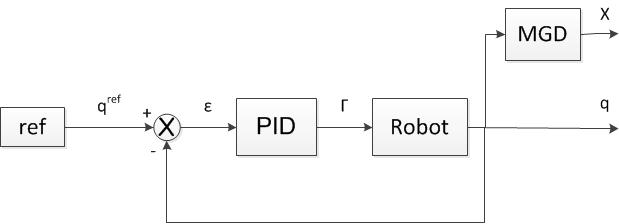
\includegraphics[width=8cm]{./PID_joint_space_bloc.JPG}
		\caption{Schéma bloc du système commandé dans l'espace angulaire par un PID}
		\label{fig:PID_joint_space_diagram}
	\end{center}
\end{figure}
	
\begin{equation} 
	 H_i(p) = \dfrac{q_i(p)}{q_{i_{ref}}(p)} = \dfrac{K_{d_i}p^2 + K_{p_i}p + K_{i_i}}{a_ip^3 + (K_{d_i} + F_{v_i})p^2 + K_{p_i}p + K_{i_i}}
	 \label{bf_PID_ang}
\end{equation}

À partir de la fonction de transfert en boucle fermée, on trouve que l'équation caractéristique du système commandé dasn l'espace angulaire par un PID est $ d(p)$ = $a_ip^3 + (K_{d_i} + F_{v_i})p^2 + K_{p_i}p + K_{i_i} $. On peut choisir, pour chaque axe, $ K_{p_i} $, $ K_{d_i} $ et $ K_{i_i} $ pour fixer la dynamique du robot en boucle fermée \cite{ogata2010modern}. On veut que le dépassement de la réponse indicielle du système en boucle fermée soit nul, alors on a besoin que $ d(p)$ = $ a_i(p + \omega_i)^3 $, où $ \omega_i $ est la pulsation de brisure en boucle fermée, choisi de façon à contrôler le temps de réponse du système. Cependant, il y a un compromis dans le choix des $ \omega_i $, parce que s'ils sont petits, le système sera trop lent, mais s'ils sont trop importants, on peut arriver à la fréquence de résonance du système due aux élasticités non modélisés du robot, et cela peut générer des signaux de commande d'amplitude très important et aussi très bruité en présence de bruit dans le système. Un bon compromis est de choisir $ \omega_i $ comme la moitié de la pulsation de résonance de l'axe i. Alors, une fois que $ \omega_i $ soit défini, on peut calculer les gains $ K_{p_i} $, $ K_{d_i} $ et $ K_{i_i} $ du PID selon les formules suivantes: 

	\begin{subequations}
	\begin{equation}
		K_{p_i} = 3a_i(\omega_i)^2
	\end{equation}
	\begin{equation}
	K_{d_i} = 3a_i(\omega_i) - F_{v_i}\\
	\end{equation}
	\begin{equation}
	K_{i_i} = a_i(\omega_i)^3
	\end{equation}
	\end{subequations}
	
Les matrices de gain du PID $ \bm{K_p} $, $ \bm{K_d} $, $\bm{K_i} \in \mathbb{R}^{n \times n}$ sont des matrices diagonales, où les éléments non nulles (i,i) sont respectivement $ K_{p_i} $, $ K_{d_i} $ et $ K_{i_i} $.
\newline

\textbf{Commande angulaire par couple calculé}
\newline

La commande par couple calculé s'agit de compensé les non-linéarités du modèle dynamique du robot par l'estimation de la matrice d'inertie $ \bm{\hat{A}}(\bm{q}) \in \mathbb{R}^{n \times n} $ et du vecteur des couples dissipatifs $ \hat{\bm{H}}(\bm{q},\dot{\bm{q}}) \in \mathbb{R}^n $. Alors, on utilisera ces paramètres pour calculé les couples selon la relation suivante, où $ \bm{w}(t) \in \mathbb{R}^n $ est une variable de commande:

	\begin{equation}
		\bm{\Gamma} = \bm{\hat{A}}(\bm{q})*\bm{w} + \hat{\bm{H}}(\bm{q},\dot{\bm{q}})
	\end{equation}

Si $  \bm{\hat{A}} $ et $ \hat{\bm{H}} $ modélisent bien la dynamique du robot et on a $ \bm{w}(t) = \ddot{\bm{q}}(t) $, cela correspond exactement au modèle dynamique direct. Avec cette loi de commande, on peut calculer le couple nécessaire pour mettre le robot dans la configuration angulaire qu'on veut avant de l'alimenter dans le robot. 

Si on utilise une loi de commande PID pour obtenir obtenir $ \bm{w}(t) = \ddot{\bm{q}}(t) $ à partir de l'erreur de position angulaire, qui est définit comme dans le cas précédent ($ \bm{\epsilon}(t) = \bm{q_{ref}}(t) - \bm{q}(t) $), et étant $ \bm{K_p} $, $ \bm{K_d} $ et $ \bm{K_i} \in \mathbb{R}^{n \times n} $ les matrices diagonales des gains du PID, on obtient:


	\begin{equation}
		\bm{w}(t) = \bm{\ddot{q}_{ref}}(t) + \bm{K_p}(\bm{q_{ref}}(t) - \bm{q}(t)) + \bm{K_d}(\bm{\dot{q}_{ref}}(t) - \bm{\dot{q}}(t)) + \bm{K_i}\int_0^t (\bm{q_{ref}}(t) - \bm{q}(t))d\tau
	\end{equation}
	
	
On peut développer cette équation dans le domaine de Laplace en fonction de l'erreur de position, sachant que $ \bm{w}(t) = \ddot{\bm{q}}(t) $: 

\begin{subequations}
\begin{equation*}
  (\bm{\ddot{q}_{ref}}(t) - \bm{\ddot{q}}(t)) + \bm{K_p}(\bm{q_{ref}}(t) - \bm{q}(t)) + \bm{K_d}(\bm{\dot{q}_{ref}}(t) - \bm{\dot{q}}(t)) + \bm{K_i}\int_0^t (\bm{q_{ref}}(t) - \bm{q}(t))d\tau = 0
\end{equation*} 
\begin{equation*}
  \bm{\ddot{\epsilon}}(t) + \bm{K_p}\bm{\epsilon}(t) + \bm{K_d}\bm{\dot{\epsilon}}(t) + \bm{K_i}\int_0^t\bm{\epsilon}(t)d\tau = 0
\end{equation*}
\begin{equation*}
 p^3\bm{\Epsilon}(p)+ p^2\bm{K_d}\bm{\Epsilon}(p) +p\bm{K_p}\bm{\Epsilon}(p) + \bm{K_i}\bm{\Epsilon}(p)=  p^2\bm{\epsilon}(0)+ p\bm{\dot{\epsilon}}(0) +\bm{\epsilon}(0)
\end{equation*} 
\end{subequations} 

Alors, cette méthode nous a permi de linéarisé l'équation de la loi de commande. Cela rend plus facile la détermination des gains du PID pour avoir les performances désirées en boucle fermée. On peut écrire l'équation de l'erreur dans le domaine de Laplace pour chaque axe, ce qui nous permet de déterminer la dynamique du système en boucle fermée \cite{ogata2010modern}:

\begin{equation}
		\Epsilon_i(p) = \dfrac{p^2\epsilon_i(0) + p(\epsilon_i(0) + \dot{\epsilon}_i(0))}{p^3 + K_{d_i}p^2 + K_{p_i}p + K_{i_i}}  
	\end{equation}

Comme il a été dit, on veut que le dépassement de la réponse indicielle soit nulle, et pour une pulsation de brisure en boucle fermée $ \omega_i $, on a:

\begin{subequations}
	\begin{equation}
		K_{p_i} = 3\omega_i^2
	\end{equation}
	\begin{equation}
		K_{d_i} = 3\omega_i
	\end{equation}
	\begin{equation}
		K_{i_i} = \omega_i^3
	\end{equation}
\end{subequations}

Dans la figure suivante, on a le schéma bloc de cette méthode de commande angulaire.

\begin{figure}[H]
	\begin{center}
		\captionsetup{justification=centering,margin=1cm}	
		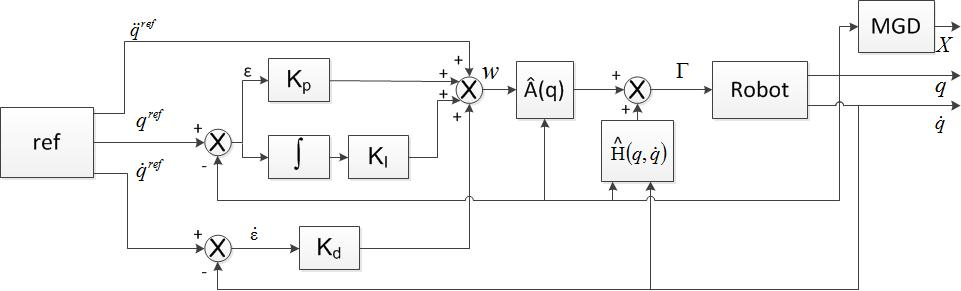
\includegraphics[width=\textwidth]{./CTI_joint_space_bloc.JPG}
		\caption{Schéma bloc du système commandé en espace angulaire par couple calculé}
		\label{fig:CTI_joint_space_diagram}
	\end{center}
\end{figure}

\subsubsection{Commande Opérationnelle}\label{Comm_Cart}

Comme pour le commande dans l'espace articulaire, il existe déjà plusieurs façon de faire la commande dans l'espace opérationnel, soit pour une approche fréquentielle, soit pour une approche temporelle. Pour question de simplicité, on a décidé d'étudier juste les approches fréquentielles. Parmi tous les méthodes fréquentielles, on étudié quatre: la commande PID opérationnelle, la commande opérationnelle par couple calculé, la commande cascade avec boucle interne de vitesse angulaire et la commande par le modèle géométrique inverse (MGI).

Dans la suite, on va présenter juste les deux derniers méthodes, avec lesquelles on a obtenu des performances les plus satisfaisantes. La commande PID opérationnelle est la plus simple, mais les lois de commande qu'on obtient sont non linéaires, ce qui rend très difficile de régler les gain du PID pour avoir des performances désirées, alors on l'a supprimé. Pour la commande opérationnelle par couple calculé, on a besoin de calculer des paramètres qui sont très instables et bruités, comme la dérivé et la pseudo-inverse de la matrice Jacobien du système, qui sera expliquée dans la suite. Ces opérations, en plus de coûteuses en ressources informatiques, apportent des imprécisions à la réponse du système et affectent ses performances, alors on l'a supprimé aussi.

À propos des autres deux méthodes de commande, ils sont équivalents par rapport aux performances et au temps de calcul numérique. Par contre, la commande cascade avec boucle interne de vitesse angulaire est plus robuste, exactement pour utiliser deux boucle de commande: une boucle externe pour la commande de position de l'outil et une boucle interne pour la commande en vitesse angulaire du robot. C'est l raison dont on a choisi d'utiliser cette commande dans notre application.
\newline

\textbf{Commande cascade avec boucle interne de vitesse angulaire}
\newline

Comme il a déjà été dit, dans ce méthode on va contrôler le robot dans l'espace opérationnel en utilisant deux boucles de commande: la boucle interne sert à commander le robot en vitesse angulaire ($\bm{\dot{q}}$), et la boucle externe sert à commander la position et l'orientation de l'outil du robot \cite{KELLY20051423}.

Pour comprendre la boucle externe, on imagine que la commande de la boucle interne est bien réglée, c'est à dire que si la boucle interne reçoit comme consigne $ \bm{\dot{q}_{ref}} $, on aura comme sortie $ \bm{\dot{q}} = \bm{\dot{q}_{ref}} $. De plus, quand on fait la commande opérationnelle du robot, il faut souvent convertir les variables de l'espace opérationnel à l'espace angulaire. Pour faire ce conversion, on utilise le Jacobien. Le Jacobien est une matrice formée par les dérivées partielles du MGD par rapport à chaque articulation du robot. Il est défini par la relation:

\begin{equation}
	\mathbb{V}_{o} = \bm{J}_{tot}(\bm{q})\bm{\dot{q}}
\end{equation}

$ \mathbb{V}_{o} = (V_{x_{o}}, V_{y_{o}}, V_{z_{o}}, \omega_{x_{o}}, \omega_{y_{o}}, \omega_{z_{o}})^T $ est le torseur cinématique, où les trois premiers termes représentent la vitesse en X, Y et Z de l'outil par rapport au repère dans la base du robot et les trois derniers termes représentent la vitesse de rotation du repère défini dans l'outil par rapport au repère dans la base du robot, autour de X, Y et Z. Pour un robot à n degrés de liberté, $ \bm{J}_{tot}(\bm{q}) \in \mathbb{R}^{6 \times n} $ est le Jacobien. On peut simplifier cette expression si on prend la vitesse de l'outil $\bm{\dot{X}} = (V_{x_{o}}, V_{y_{o}}, V_{z_{o}})^T$ au lieu du torseur cinématique, et le Jacobien devient $\bm{J} = \bm{J}_{tot}(1:3,:)$, $ \bm{J} \in \mathbb{R}^{3 \times n} $. Alors, on peut écrire les équations: 

\begin{subequations}
	\begin{equation}
		\bm{\dot{X}} = \bm{J}(\bm{q})\bm{\dot{q}}
		\label{MCD}
	\end{equation}
	\begin{equation}
		\bm{\dot{q}} = \bm{J}^{\ast}(\bm{q})\bm{\dot{X}}
	\end{equation}
\end{subequations}

Où $ \bm{J}^{\ast} = \bm{J}^T(\bm{J}\bm{J}^T)^{-1} $ est la pseudo inverse du Jacobien. 

Soit $ \bm{X}_{ref} $ et $ \bm{\dot{X}}_{ref} $ les réferences de position et vitesse respectivement pour l'outil du robot, $ \bm{\epsilon_X} =  \bm{X}_{ref} - \bm{X} $ l'erreur de position de l'outil, K un gain et $ \bm{\omega}_{ref} $ la réference de vitesse angulaire qui sera fourni à la boucle interne, on défine la loi de commande de la boucle externe:

\begin{equation}
	\bm{\omega}_{ref} = \bm{J}^{\ast}(\bm{\dot{X}}_{ref} + K\bm{\epsilon})
	\label{comm_cascade}
\end{equation}

Le schéma bloc de la boucle externe de cette méthode de commande est montré dans la figure \ref{fig:cascade_outer_diagram}.

\begin{figure}[H]
	\begin{center}	
		\captionsetup{justification=centering,margin=1cm}
		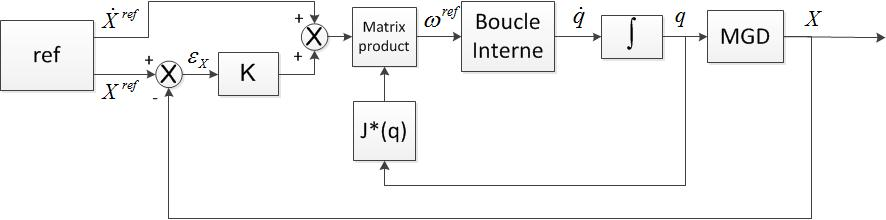
\includegraphics[width=\textwidth]{./cascade_outer_diagram.JPG}
		\caption{Schéma bloc de la boucle externe du commande cascade}
		\label{fig:cascade_outer_diagram}
	\end{center}
\end{figure}

Si on a une boucle interne bien réglée $ (\bm{\dot{q}} = \bm{\omega}_{ref}) $, on multiplie l'équation \ref{comm_cascade} par $ \bm{J} $ et on utilise la relation \ref{MCD}, on obtient:

\begin{equation}
	\bm{\dot{\epsilon}_X} = - K\bm{\epsilon_X}
	\label{cascade_error}
\end{equation}

Alors, on peut voir dans la relation \ref{cascade_error} que l'erreur tend à zéro de façon exponentielle avec une constant de temps K qui nous permet de contrôler la dynamique du système. Mais pour que la boucle externe fonctionne, on doit bien régler la boucle de vitesse angulaire.

Pour faire la commande de la boucle interne, on utilise la méthode du couple calculé, comme décrite dans la section \ref{Comm_Ang}, mais au lieu de fixer des consignes de position angulaire, on fixe des consignes de vitesse angulaire. On dénife la loi de commande dans l'équation suivant.

\begin{subequations}
	\begin{equation}
		\bm{\Gamma} = \bm{\hat{A}}(\bm{q})*\bm{w} + \hat{\bm{H}}(\bm{q},\dot{\bm{q}})
	\end{equation}
	\begin{equation}
		\bm{w} = \bm{\dot{\omega}}_{ref} + K_p\bm{\epsilon_{\dot{q}}} + K_i\int_0^t {\epsilon_{\dot{q}}}d\tau = \bm{\ddot{q}}
	\end{equation}
\end{subequations}

Où $ \bm{\epsilon_{\dot{q}}} = \bm{\omega}_{ref} - \bm{\dot{q}} $ est l'erreur de vitesse angulaite du robot et $ K_p $ et $ K_i $ sont deux gain utilisés pour reglé la dynamique de la boucle de vitesse, équivalents à une commande PI (\textit{Proportional Integral}).

Le schéma bloc de la boucle interne de cette méthode de commande est montré dans la figure \ref{fig: cascade_inner_diagram}.

\begin{figure}[H]
	\begin{center}	
		\captionsetup{justification=centering,margin=1cm}
		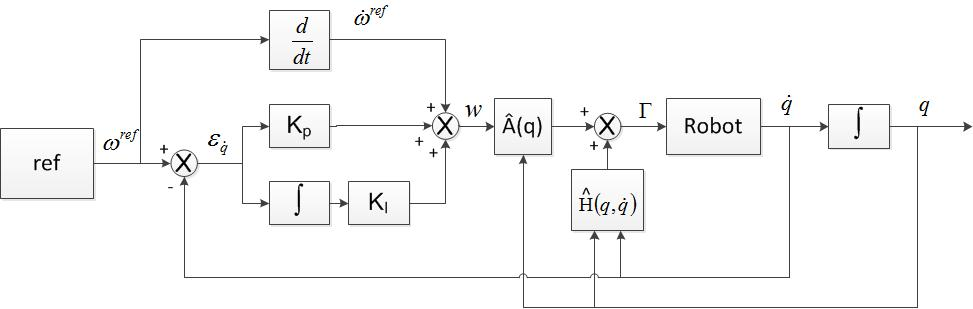
\includegraphics[width=\textwidth]{./cascade_inner_diagram.JPG}
		\caption{Schéma bloc de la boucle interne du commande cascade}
		\label{fig: cascade_inner_diagram}
	\end{center}
\end{figure}


\textbf{Commande opérationnelle par le modèle géometrique inverse (MGI)}
\newline

Le MGI sert à convertir une configuration (position plus orientation) faisable de l'outil du robot à des angles des articulations qui laissent l'outil dans cette configuration. Si on a le MDI, on peut faire la commande du robot dans l'espace opérationnel en utilisant le schéma de commande angulaire (comme par exemple, celle de la figure \ref{fig:PID_joint_space_diagram}), parce qu'on convertit les consignes de position aux consignes angulaires. Le problème est que générer le MDI n'est pas facile, et parfois il y a plus d'une configuration angulaire qui conduit à la configuration de l'outil qu'on veut.

Pour dévelloper le MDI, on s'est basé sur la méthode \textit{Yasukawa Motomart L-3} \cite{craig2005introduction}. Premièrement, on doit écrire les matrices homogènes de changement de repère d'une axe du robot à l'axe suivante \cite{khalil2004modeling}. Soit $\bm{T}_{i,j}$ la matrice de changement du repère de l'axe i au repère de l'axe j (end répresent le repère de l'outil du robot), $d_i$ la distance du repère i au repère (i-1) par rapport à l'axe X du repère (i-1), $r_i$ la distance du repère i au repère (i-1) par rapport à l'axe Z du repère (i-1) et $ \theta_i $ est la position angulaire de l'axe i, on trouve les matrices de changement de repère selon le diagramme physique du robot \cite{YoubotKin}:

\begin{multicols}{2}	
	\begin{equation*}
		\bm{T}_{0,1} = \left[\begin{array}{cccc} cos(\theta_1) & -sin(\theta_1) & 0 & d_1 \\ sin(\theta_1) & cos(\theta_1) & 0 & 0 \\ 0 & 0 & 1 & r_1 \\ 0 & 0 & 0 & 1 \end{array}\right]
	\end{equation*}
	
	\begin{equation*}
		\bm{T}_{1,2} = \left[\begin{array}{cccc} cos(\theta_2) & -sin(\theta_2) & 0 & d_2 \\ 0 & 0 & -1 & 0 \\ sin(\theta_2) & cos(\theta_2) & 0 & 0 \\ 0 & 0 & 0 & 1 \end{array}\right]
	\end{equation*}	
	
	\begin{equation*}
		\bm{T}_{2,3} = \left[\begin{array}{cccc} cos(\theta_3) & -sin(\theta_3) & 0 & d_3 \\ sin(\theta_3) & cos(\theta_3) & 0 & 0 \\ 0 & 0 & 1 & 0 \\ 0 & 0 & 0 & 1 \end{array}\right]
	\end{equation*}	
	
	\begin{equation*}
		\bm{T}_{3,4} = \left[\begin{array}{cccc} cos(\theta_4) & -sin(\theta_4) & 0 & d_4 \\ sin(\theta_4) & cos(\theta_4) & 0 & 0 \\ 0 & 0 & 1 & 0 \\ 0 & 0 & 0 & 1 \end{array}\right]
	\end{equation*}	
	
	\begin{equation*}
		\bm{T}_{4,5} = \left[\begin{array}{cccc} cos(\theta_5) & -sin(\theta_5) & 0 & 0 \\ 0 & 0 & 1 & 0 \\ -sin(\theta_5) & -cos(\theta_5) & 0 & 0 \\ 0 & 0 & 0 & 1 \end{array}\right]
	\end{equation*}	
	
	\begin{equation*}
		\bm{T}_{5,end} = \left[\begin{array}{cccc} 1 & 0 & 0 & 0 \\ 0 & 1 & 0 & 0 \\ 0 & 0 & 1 & l_{end} \\ 0 & 0 & 0 & 1 \end{array}\right]
	\end{equation*}	
\end{multicols}

On sait que, pour obtenir la matric de changement du repère i au repère k étant données $ \bm{T}_{i,j} $ et $ \bm{T}_{j,k} $, il suffit de faire $ \bm{T}_{i,k} = \bm{T}_{i,j} * \bm{T}_{j,k} $. Alors, avec les matrices de changement de repère du robot, on peut trouver la relation suivante:

\begin{equation}
	\bm{T}_{1,5} = \bm{T}_{0,1}^{-1} * \bm{T}_{0,5} = \bm{T}_{1,2} * \bm{T}_{2,3} * \bm{T}_{3,4} * \bm{T}_{4,5}
	\label{MDI_rel1}
\end{equation}
	
Soit $ \bm{T}_{0,5} $ la configuration du repère de l'axe 5 par rapport à la base du robot, qu'on peut trouver à partir de la configuration désirée pour l'outil $ \bm{T}_{0,end} $ avec la relation $ \bm{T}_{0,5} = \bm{T}_{0,end} * \bm{T}_{5,end}^{-1} $, définie par:

\begin{equation}
	\bm{T}_{0,5} = \left[\begin{array}{cccc} r_{1,1} & r_{1,2} & r_{1,3} & p_x \\ r_{2,1} & r_{2,2} & r_{2,3} & p_y \\ r_{3,1} & r_{3,2} & r_{3,3} & p_z \\ 0 & 0 & 0 & 1 \end{array}\right]
\end{equation}
\pagebreak\\
Alors, on obtient de \eqref{MDI_rel1}:

\begin{equation}
	\left[\begin{array}{cccc} * & * & r_{1,3}c1 + r_{1,3}s1 & * \\ r_{2,1}c1 - r_{1,1}s1 & r_{2,2}c1 - r_{1,2}s1 & * & k_1 \\ * & * & r_{3,3} & * \\ 
	0 & 0 & 0 & 1 \end{array}\right] = \left[\begin{array}{cccc} * & * & -s234 & * \\ s5 & c5 & * & 0 \\ * & * & c234 & * \\ 0 & 0 & 0 & 1 \end{array}\right]
\end{equation}

Où $c1 = cos(\theta_1)$, $s1 = sin(\theta_1)$, $s234 = sin(\theta_2 + \theta_3 + \theta_4)$, $c234 = cos(\theta_2 + \theta_3 + \theta_4)$, $c5 = cos(\theta_5)$, $s5 = sin(\theta_5)$, et $k_1 = p_yc1 - (p_x - d_1)s1$.

Pour comparaison des deux matrices dans la relation précédente, on trouve déjà que:
\begin{subequations}
	\begin{equation}
		\theta_1 = atan2(p_y, p_x - d_1)
	\end{equation}
	\begin{equation}
		\theta_5 = atan2(r_{2,1}cos(\theta_1) - r_{1,1}sin(\theta_1), r_{2,2}cos(\theta_1) - r_{1,2}sin(\theta_1))
	\end{equation}
	\begin{equation}
		\theta_2 + \theta_3 + \theta_4 = atan2(-(r_{1,3}cos(\theta_1) - r_{2,3}sin(\theta_1)), r_{3,3})
	\end{equation}
\end{subequations}

Maintenant, pour trouver les angles $ \theta_2 $ et $ \theta_3 $ on doit utiliser une approche géométrique. Si on observe d'un repère situé sur l'axe 2 du robot (ce qu'on peut faire parce que, une fois qu'on a $ \theta_1 $, il suffit d'obtenir $ \bm{T}_{1,5} $ et de faire une translation de $-d_2$ par rapport à l'axe X pour obtenir $ \bm{T}_{proj2} $), la position de l'axe 5 est défini comme dans la figure \ref{fig:MDI_rel2}, où $ \overline{p_x}$, $\overline{p_y}$ et $\overline{p_z}$ sont, respectivent, les élements (1,4), (2,4) et (3,4) de la de matrice $ \bm{T}_{proj2} $.

\begin{figure}[H]
	\begin{center}	
		\captionsetup{justification=centering,margin=1cm}
		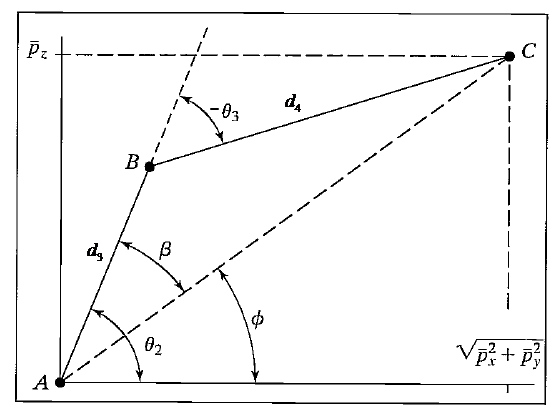
\includegraphics[width=8cm]{./MDI_rel2.PNG}
		\caption{Configuration du robot youBot KUKA vue de l'articulation 2.}
		\label{fig:MDI_rel2}
	\end{center}
\end{figure}

Si on applique la loi des cossinus, on peut trouver les angles $ \theta_2 $ et $ \theta_3 $, selon les équations suivantes. Une fois qu'on a ces deux angles et on a aussi $(\theta_2 + \theta_3 + \theta_4)$, on peut obtenir facilement le $ \theta_4 $ et de cette façon, on a retrouvé tous les angles.
\pagebreak
\begin{subequations}
	\begin{equation}
		cos(-\theta_3) = \dfrac{\overline{p_x}^2 + \overline{p_y}^2 + \overline{p_z}^2 - d_3^2 - d_4^2}{2d_3d_4}
	\end{equation}
	\begin{equation}
		\theta_3 = - atan2(\sqrt{1 - cos^2(-\theta_3)}, cos(-\theta_3))
	\end{equation}
	\begin{equation}
		\theta_2 = atan2(\overline{p_z}, \sqrt{\overline{p_x}^2 + \overline{p_y}^2}) + atan2(r_4sin(\theta_3), r_3 + r_4cos(\theta_3))
	\end{equation}
\end{subequations}

Il est possible pour le robot de atteint une position désirée avec le coude haut ou bas et avec la poignée haute ou basse, alors quatre configurations angulaires différentes pour la même position. Avec cette méthode, on peut retrouvé la configuration coude bas et poignée basse par défaute. Si on veut changer la configuration, il suffit d'ajouter ou de soustraire un décalage de $ \pi $ à l'axe 1 pour le coude et à l'axe 3 pour la poignée.

Le problème que nous reste à propos de ce modèle est qu'il marche juste si on essai une configuration faisable de l'outil. Comme le robot youBot KUKA a 5 dégrés de libertés, une fois qu'on a fixé la position de l'outil, il ne peut pas avoir n'importe quelle orientation para rapport à la base du robot. En fait, La position fixé pour l'outil fixe aussi le plan ou le bras du robot va rester par l'angle $ \theta_1 $. Alors, juste les orientation dont l'axe Z du repère situé dans l'outil est contenue dans ce plan sont faisables.

Pour éviter ce problème, on a décidé de faire tous les trajectoires du robot au cours du Jeu avec l'outil tourné vers l'avant. Il est facile de déterminer pour n'importe quelle position quelle est l'orientation qui correspond à l'outil vers l'avant. Dans le repère de la première articulation, les axes X et Z déterminent le plan du bras du robot. Par rapport à cette repère, si on veut fixer cette orientation, on a besoin d'utiliser la matrice de rotation suivante:

\begin{equation*}
	\bm{R_{avant}} = \left[\begin{array}{ccc} 0 & 0 & 1 \\ 0 & 1 & 0 \\ -1 & 0 & 0 \end{array}\right]
\end{equation*}

Comme juste la position de l'outil défine l'angle $ \theta_1 $, il suffit pour construire $ \bm{T}_{0,1} $. Alors, on peut rajouter $ \bm{R_{avant}} $ à la position désirée pour obtenir la matrice homogène $ \bm{T}_{1,end} $ avec une cofiguration faisable pour l'outil et revenir au repère de la base en multipliant cette matrice pour $ \bm{T}_{0,1}^{-1} $.